\section{Description technique}

\subsection{Structure}
\subsubsection{Structure de JavaFX}
Notre application se base sur la structure officielle d'une application JavaFX, qui se prête parfaitement à notre type d'application. Sa compréhension est essentielle pour discuter de l'architecture de notre logiciel.
\par
Les trois point-clés sont la notion de \texttt{\gls{stage}}, de \texttt{\gls{scene}} et de \gls{scene_graphe}. Le \texttt{Stage} est le container haut-niveau d'une application JavaFX \cite{javadoc_stage}. Il doit contenir tout le contenu d'une fenêtre. La \texttt{Scene} est le container pour un Scene Graph. Chaque \texttt{Scene} doit avoir un et un seul n\oe ud racine du Scene Graph \cite{javadoc_scene}.
\par
Le Scene Graph est une structure en arbre qui garde une représentation interne des éléments graphiques de l'application. En tout temps, il sait quels éléments afficher, quelles zones de l'écran doivent être rafraîchies, et comment le faire de la manière la plus efficace \cite{javadoc_scene_graphe}. 	

\begin{figure}[H]
	\caption{Représentation du Scene Graph de JavaFX. Source: documentation Oracle \cite{javadoc_scene_graphe}}
	\centering
	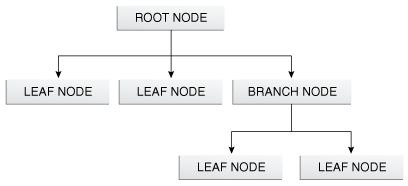
\includegraphics[scale=0.6]{scene_graphe_1.png}
	\label{fig:scene_graphe_1}
\end{figure}
Comme on peut le voir sur la figure \ref{fig:scene_graphe_1}, chaque n\oe ud de l'arbre du Scene Graph appartient à la hiérarchie de la classe \texttt{\gls{node}}. De plus, chacun de ces n\oe uds est soit une feuille (ne pouvant pas contenir d'enfants), soit une branche (pouvant alors contenir des enfants).
\par
Cette structure particulière permet donc de créer facilement des interfaces graphiques, car il suffit que chaque élément visuel de notre application soit un objet (spécialisé ou non) d'une classe héritant de \texttt{Node} pour que l'affichage de cet élément soit géré automatiquement par JavaFX.
\par
Pour beaucoup de nos composants, nous avons donc spécialisé une des classes offertes par JavaFx proposant la fonctionnalité recherchée, en y ajoutant les comportements dont nous avions besoin. Ils sont ensuite ajoutés au Scene Graph de la scène principale, et nous pouvons ainsi construire notre application.

\subsection{Serialisation}
\label{sec:serialisation}

En Java, la sérialisation s'effectue à l'aide de l'interface \texttt{Serializable}. Par conséquent, chaque classe de Java implémentant cette dernière telle que \texttt{String}, peut être sérialisée et désérialisée à volonté. Cependant, la majorité des classes JavaFX n'implémentent pas cette interface. En effet, cette librairie utilise grandement des mécanismes et des liaisons dynamiques tel que les listeners qui sont pour l'instant des sous-systèmes non-sérialisables. C'est pourquoi JavaFX contient très peu d'objets sérialisables.

Pour combler ce manque, nous devons nous-mêmes implémenter la sérialisation des classes JavaFX que nous sommes susceptibles d'utiliser.

\begin{figure}[h]
    \caption{Diagramme de la sérialisation simplifié}
    \centering
    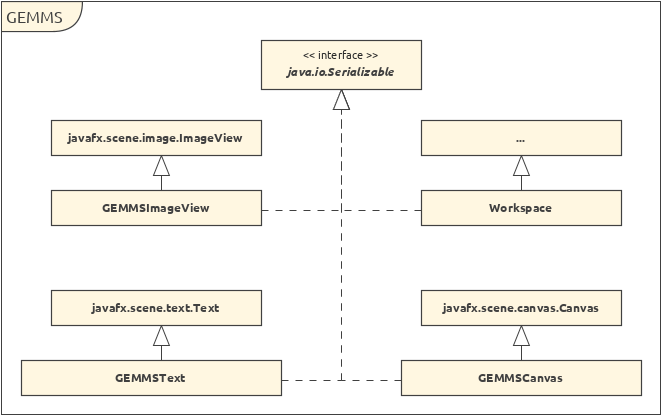
\includegraphics[scale=0.6]{serialisation_diagram.png}
    \label{fig:seri_diag}
\end{figure}

Sur la figure \ref{fig:seri_diag}, nous pouvons voir un diagramme simplifié de l'implémentation de la sérialisation. Dans notre application, nous allons utiliser des classes de base telles que \texttt{\gls{imageview}}, \texttt{\gls{text}}, \texttt{\gls{canvas}}, \texttt{Color}, etc. Nous devons donc spécialiser ces classes afin qu'elles puissent implémenter l'interface \texttt{Serializable}. Toutefois, certaines classes comme \texttt{Color} ne sont malheureusement pas spécialisables. Il faut donc sérialiser les paramètres un par un à l'aide des accesseurs et mutateurs de cette dernière.

Étant donné que les classes JavaFX possèdent énormément de fonctionnalités, sérialiser l'entier de celles-ci nous demanderait beaucoup trop de temps. C'est pourquoi nous nous contentons uniquement des paramètres utilisés au sein du projet tel que la largeur, la hauteur, la position, etc.

\lstinputlisting[language=Java, caption=Exemple de sérialisation]{./src/serialisation.java}

Bien que la sérialisation soit possible, ceci engendre des contraintes et des pertes de performances. Par exemple, les classes spécialisées ne peuvent plus étendre d'une classe commune et bénéficier de ses méthodes. De plus, les objets comme \texttt{Canvas} et \texttt{ImageView} devront sérialiser pixel par pixel, ce qui peut être long et volumineux selon la taille.

\subsection{Sauvegarde}
La sauvegarde d'un document utilise la sérialisation des objets. Comme mentionné précédemment, la sérialisation de certaines classes peut être volumineux. Ainsi, les données sont compressées dans le format GZIP.

\subsection{Workspace et liste des calques}
Le \texttt{\gls{workspace}} correspond à l'espace de travail d'un Document GEMMS. \texttt{Workspace} est une classe personnalisée héritant de la classe \texttt{StackPane} de JavaFX. 

\subsubsection{Structure d'un Workspace}
Chaque document ouvert possède un objet \texttt{Workspace} permettant à l'utilisateur de manipuler le contenu du fichier. Il est constitué de plusieurs couches de composants, comme représenté sur la figure \ref{fig:workspace_representation}.


\begin{figure}[H]
	\caption{Représentation des couches du \texttt{Workspace}}
	\centering
	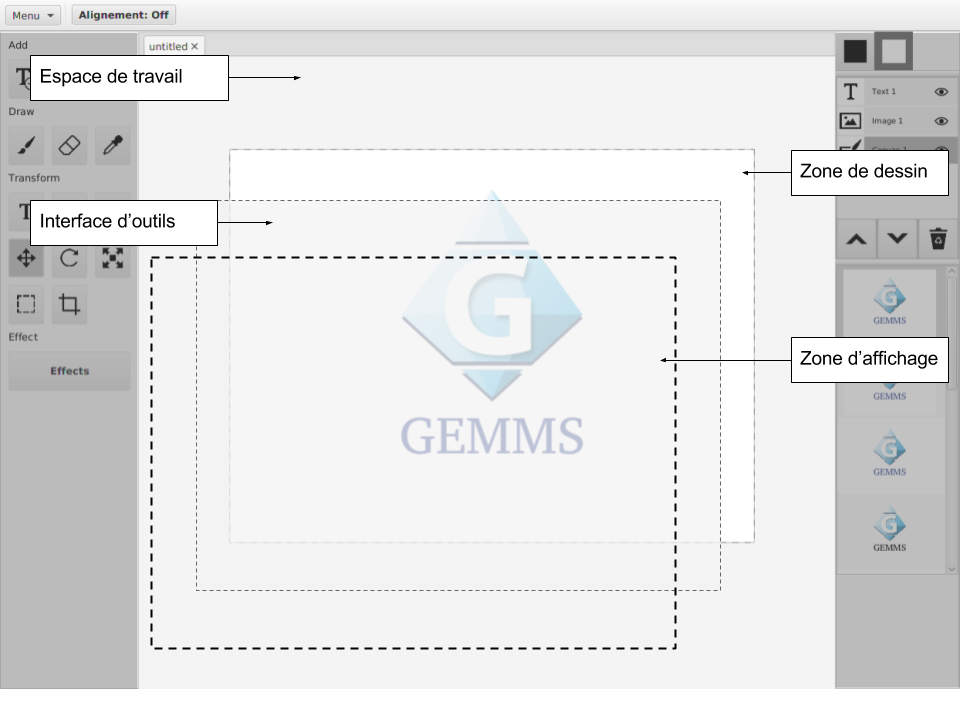
\includegraphics[scale=0.4]{workspace_schema.png}
	\label{fig:workspace_representation}
\end{figure}

L'espace de travail (\texttt{Workspace}) est un container contenant deux enfants (au sens de l'arbre de JavaFX): une zone de dessin (une branche du Scene Graph) où sont ajoutés tous les calques créés et modifiés par l'utilisateur, et une interface des outils permettant de dessiner les retours visuels des outils (comme le curseur du pinceau par exemple). Tous deux sont de type \texttt{\gls{anchorpane}}, un type spécifique de container JavaFX, car cette classe permet de positionner leurs enfants selon des coordonnées (x, y).

La zone d'affichage correspond à un masque appliqué à l'espace de travail pour éviter que les calques ne dépassent de la zone dessin. En effet les parents de type \texttt{AnchorPane} ne cachent pas leur éléments enfants sortant de leurs frontières.

Le \texttt{Workspace} détecte les mouvements de souris sur l'interface des outils et se charge d'appeler les méthodes correspondantes de l'objet \texttt{Tool} activé (se référer à la section \ref{section_outils}).

\subsubsection{Types de calques}
Dans GEMMS, les éléments d'un document sont gérés au moyen de calques. L'application utilise trois sortes de calques, qui sont en fait des types de \texttt{Node} proposés par JavaFX. La classe \texttt{\gls{text}} permet de représenter des textes, la classe \texttt{\gls{canvas}} permet de dessiner des éléments graphiques (lignes, formes, etc.) et la classe \texttt{\gls{imageview}} permet de représenter des images. 

Pour les besoins de l'application, nous ne pouvions pas utiliser ces classes telles qu'elles sont proposées par l'API JavaFX. Nous avons donc créer des classes spécialisées (\texttt{\gls{gemmstext}}, \texttt{\gls{gemmstext}} et  \texttt{\gls{gemmsimage}}) de chacun de ces éléments afin de pouvoir ajouter les fonctionnalités nécessaires. La figure \ref{fig:layer_hierarchy} illustre cette spécialisation.

\begin{figure}[H]
	\caption{Spécialisation des classes JavaFX pour la gestion des calques}
	\centering
	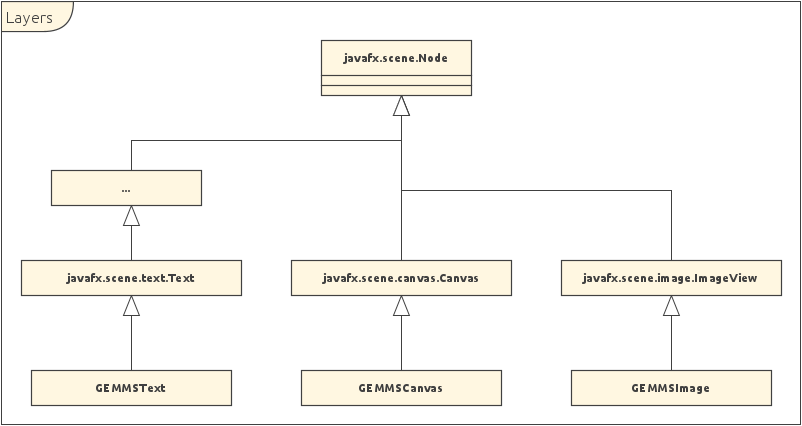
\includegraphics[scale=0.55]{layer_hierarchy.png}
	\label{fig:layer_hierarchy}
\end{figure}


\subsubsection{Gestion des calques}

Une des fonctionnalités indispensables de GEMMS est de permettre à l'utilisateur de gérer les calques de son document au moyen d'une liste dans un panneau de l'interface. Il s'agit d'une représentation visuelle de l'état du Scene Graph dans la branche de la zone de dessin dont nous parlons plus haut. Elle doit donc être en tout temps synchronisée avec l'état actuel du document et tout changement doit se répercuter dans cet affichage de calques.

La classe \texttt{ListView} de JavaFX propose cette fonctionnalité. Malheureusement, ce composant n'étant pas paramétrable comme nous le souhaitions pour les besoins ergonomiques de l'application, nous avons dû implémenter notre propre système de gestion de calques. Il est cependant fortement inspiré du fonctionnement de \texttt{ListView}.

\begin{figure}[H]
	\caption{Implémentation du composant \texttt{LayerList}. Structure simplifiée.}
	\centering
	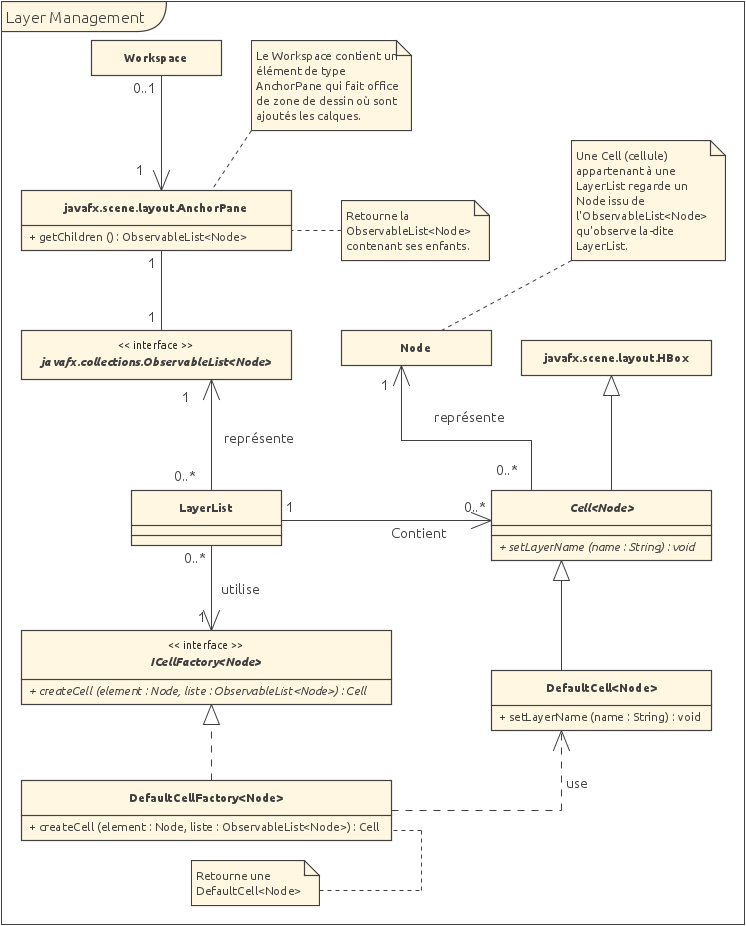
\includegraphics[scale=0.6]{layer_management.png}
	\label{fig:layer_management}
\end{figure}

\texttt{LayerList} est une classe générique implémentée pour ce projet qui permet d'afficher sous forme de liste de cellules le contenu d'une \texttt{ObservableList}. La figure \ref{fig:layer_management} illustre la structure du \texttt{Workspace} et de sa \texttt{LayerList}. Dans cette représentation, toutes les classes sont instanciées avec \texttt{Node} comme paramètre générique pour une meilleure compréhension. Les enfants d'un \texttt{Node} de type parent étant représentés sous la forme d'une \texttt{ObservableList<Node>} dans JavaFX, \texttt{Layerlist} peut ainsi gérer les calques du \texttt{Workspace}.

\texttt{LayerList} hérite du composant \texttt{VBox} de JavaFX, ce qui permet de l'ajouter au Scene Graph. Dans GEMMS, elle observe les enfants de la zone de dessin du \texttt{Workspace} et est notifiée lorsqu'il y a un changement. Pour tout nouveau calque (\texttt{Node}) ajouté dans la liste, elle crée une nouvelle \texttt{Cell} (cellule) en utilisant le pattern de fabrication abstraite. Elle ajoute ces cellules dans un composant interne qui les affiche en colonne.

Une \texttt{Cell} (cellule) est un élément \texttt{HBox} JavaFX spécialisé, qui garde trace d'un \texttt{Node} (calque du document) et qui permet de contrôler et d'afficher des information concernant ce \texttt{Node}. Chaque \texttt{Cell} peut en effet être sélectionnée, masquée, renommée, ou supprimée au clic de la souris, et ces actions se répercutent sur les calques effectifs contenus par le \texttt{Workspace}. 

Ce système de gestion permet de fournir une vue des calques qui se maintient elle-même à jour, et ce quel que ce soit les changements apportés aux à la liste d'enfants de la zone de dessin.

Le \texttt{Workspace} peut donc déléguer entièrement la gestion des calques à un objet de type \texttt{LayerList}. Les méthodes d'accès aux calques sélectionnés du \texttt{Workspace} font donc appel aux méthodes de la \texttt{LayerList}.

\lstinputlisting[language=Java, caption=Exemple de gestion de la sélection des calques par la \texttt{LayerList} au sein du \texttt{Workspace}]{./src/gestion_calques.java}

\subsection{Copier-coller}
\label{sec:copiercoller}
Deux façon d'aborder le copier-coller ont été implémentées : la première consiste à enregistrer dans le presse-papier un ou des calques sélectionnés, la seconde consiste à enregistrer uniquement la partie sélectionnée et visible à l'écran.

Trois procédés sont à l'origine de cette fonction de l'application : le snapshot, le viewport et la sérialisation.


\subsubsection{Snapshot}
Le snapshot est un outil proposé par JavaFX qui permet d'effectuer une «capture» d'un élément ou un groupe d'élément. C'est ce qui nous intéresse lorsque l'on fait une copie d'une zone sélectionnée de l'écran. L'image ainsi capturée est alors écrite sur un \texttt{GEMMSCanvas} qui est sérialisé et enregistré dans le presse-papier.

\subsubsection{Viewport}
La notion de Viewport intervient dans le cas d'un snapshot. Elle permet de définir une «fenêtre» de capture rectangulaire à laquelle se restreindra le snapshot, on la passe en paramètre au moment d'effectuer ce dernier.

Ce mécanisme est utilisé quand on copie une zone sélectionnée de l'espace de travail (voir \ref{sec:selection} pour la sélection). Les coordonnées de la sélection (position et taille) sont récupérées et utilisées pour créer un viewport. Le défi principal a été de gérer le système de coordonnées de JavaFX. En effet, chaque n\oe ud possède son propre système de coordonnées et un point de ce n\oe ud peut être exprimé selon le système de coordonnées local au n\oe ud, selon le système du parent direct du n\oe ud ou encore selon le système de la fenêtre, de l'écran etc.

La notion a maîtriser ici est d'exprimer au viewport ses dimensions dans le système de coordonnées du parent du n\oe ud sur lequel on effectue le snapshot. Une fois cette notion comprise, le snapshot est restreint au viewport (et donc à la sélection) et le comportement voulu est adopté.

Il reste ensuite à écrire l'image capturée sur un \texttt{GEMMSCanvas} qui sera affiché par la suite dans l'espace de travail.

\subsubsection{Sérialisation}
Le presse-papier ne permet d'enregistrer que des données textuelles, il faut donc sérialiser le ou les calques qui seront stockés dans le presse-papier. Pour plus de détails sur la sérialisation, voir la section \ref{sec:serialisation}.

\subsubsection{Coller le contenu du presse-papier}
Le collage consiste à désérialiser le contenu du presse-papier et à insérer dans le \texttt{Workspace} courant le ou l'ensemble de calques désérialisés.

\subsection{Historique}
L'historique des actions effectuées se base principalement sur deux concepts : la sérialisation et le patron de conception «Observable» comme l'indique la figure \ref{fig:hist_uml}.

\begin{figure}[h]
    \caption{Diagramme de l'historique simplifié}
    \centering
    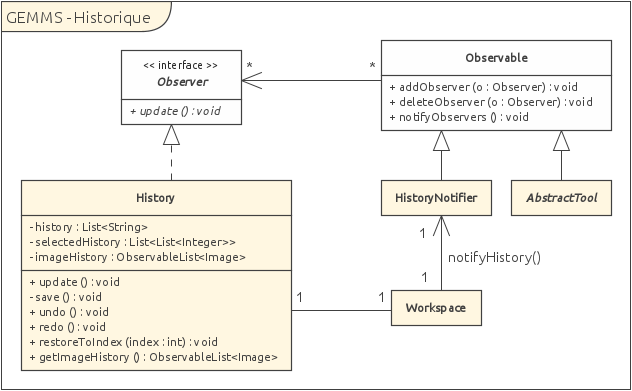
\includegraphics[scale=0.6]{history_uml.png}
    \label{fig:hist_uml}
\end{figure}

Après chaque action que l'on souhaite pouvoir annuler, on notifie l'instance de la classe \texttt{History} liée au \texttt{Workspace} en cours d'utilisation. \texttt{History} implémente donc \texttt{Observer} et observe les outils ainsi que le \texttt{HistoryNotifier}. Lorsqu'il reçoit une notification, l'historique sauvegarde l'entier du \texttt{Workspace}. C'est à ce moment qu'intervient la sérialisation. Il aurait été possible d'utiliser l'interface \texttt{Cloneable} pour les différents \texttt{GEMMSNode} et sauvegarder systématiquement des copies des objets, cependant le code aurait été très similaire à celui de la sérialisation. Nous avons donc décidé de sérialiser les calques de l'espace de travail et d'enregistrer la chaîne de caractères en résultant. Note : l'utilisation de \texttt{HistoryNotifier} se justifie par le fait que \texttt{Workspace} étend la classe \texttt{StackPane} et ne pouvait donc pas être lui-même \texttt{Observable}.

Lorsque les méthodes \texttt{undo()} et \texttt{redo()} sont appelées (notamment par les commandes Ctrl + Z et Ctrl + Y), l'historique restaure (désérialise) la sauvegarde faite dans la liste d'éléments sérialisés correspondant à l'action demandée.

De la même manière que pour les calques, la liste des calques sélectionnés au moment de la sauvegarde est enregistrée afin que lorsque l'utilisateur restaure l'état précédent, les calques qu'il avait sélectionnés le soient à nouveau.

\subsubsection{Historique visuel}
L'affichage de l'historique visuel utilise le même mécanisme que décrit ci-dessus. À chaque action de l'utilisateur, on effectue une capture («snapshot») miniature de l'espace de travail qui sera stockée dans une liste. Cette liste est observable et alimente une \texttt{ListView} qui affiche les images dans l'interface de GEMMS.

Lorsque l'utilisateur clique sur un élément de la \texttt{ListView}, la méthode \texttt{restoreToIndex(index)} de l'historique est appelée. Elle restaure l'espace de travaille non pas à l'état précédent, mais à l'état indiqué par le paramètre entier positif \texttt{index}.

On notera finalement que si l'utilisateur effectue une modification après avoir restauré un état précédent, il se trouvera sur une nouvelle «branche» et il ne pourra plus «revenir en avant», comme sur pratiquement tous les logiciels que l'on connaît, voir figure \ref{fig:hist_branches}.

\begin{figure}[h]
    \caption{Fonctionnement de l'historique}
    \centering
    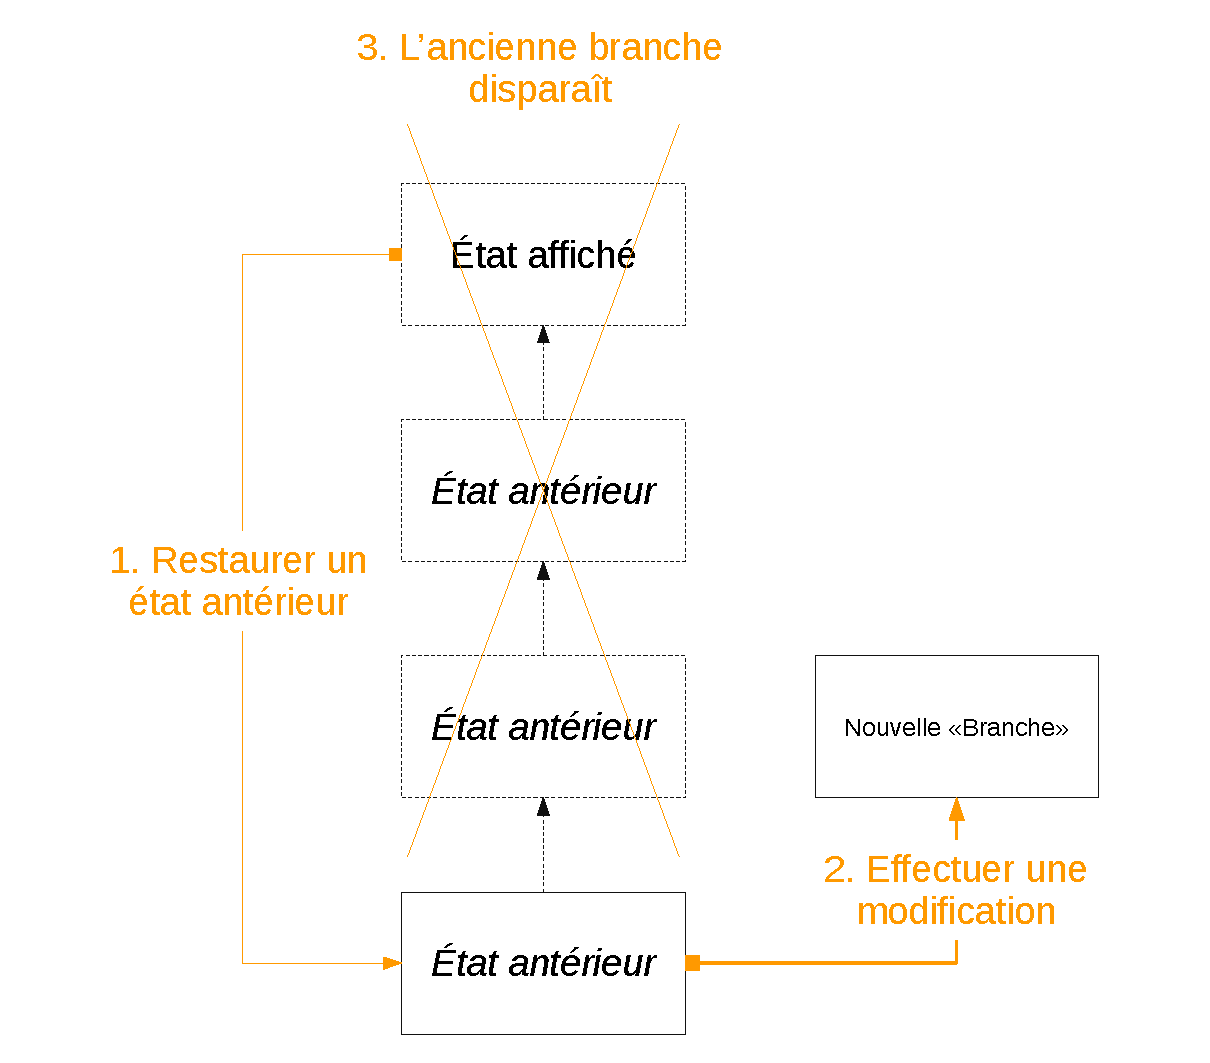
\includegraphics[scale=0.6]{history_branches.pdf}
    \label{fig:hist_branches}
\end{figure}

\subsection{Positionnement}
TODO TODO TODO

\subsection{Outils}
\par
JavaFX offre (entre autres) les événements \texttt{MousePressed}, \texttt{MouseDragged} et \texttt{MouseReleased}. Ils correspondent respectivement à l'action de presser la souris, de la déplacer en gardant le clic gauche enfoncé ou de relâcher le clic gauche de la souris.
\subsubsection{Hiérarchie des outils}
\label{section_outils}
\par
La plupart des outils de l'application  fonctionnent grâce à ces trois événements. On pensera notamment au pinceau qui doit dessiner un trait en suivant la souris lors d'un \texttt{MouseDragged}. Un quatrième événement, \texttt{MouseMouved} est également traité, mais il n'est utilisé que pour afficher des retours visuels (curseur du pinceau par exemple). Son utilisation n'est donc pas détaillée dans cette section.
\par
Comme on peut le voir sur la figure \ref{fig:tool_hier}, les outils implémentent une interface \texttt{Tool}, possédant des méthodes correspondant à ces événements. Au long de l'exécution du programme, le \texttt{Workspace} garde une référence vers un outil considéré actif (qui peut aussi être référence nulle), et lorsqu'il détecte un des événements cités plus haut, il se charge d'appeler la ou les méthodes correspondantes de cet outil.
\par
Lorsque l'utilisateur clique sur un bouton pour activer un outil, le programme crée une nouvelle instance de ce type d'outil, et le \texttt{Workspace} utilise cet outil pour traiter les événement \texttt{MousePressed}, \texttt{MouseDragged} ou \texttt{MouseReleased}.
\par
D'autres outils plus simples, comme la symétrie horizontale ou verticale ou les effets de couleurs sont implémentés en ajoutant un action à des composants de bases de JavaFX comme des \texttt{Button} ou des \texttt{Slider}.

\begin{figure}[H]
	\caption{Diagramme simplifié de la hiérarchie des outils}
	\centering
	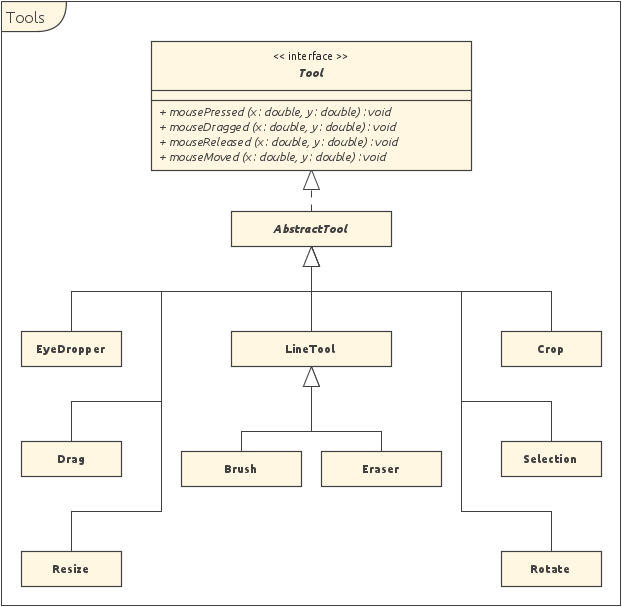
\includegraphics[scale=0.6]{tool_hierarchy.png}
	\label{fig:tool_hier}
\end{figure}

\subsubsection{Réglage des outils} \label{reglage-outils}
Certains de ces outils nécessitent d'être paramétrés en temps réel en fonction des calques sélectionnés par l'utilisateur. Par exemple, la taille de la gomme est stockée dans l'objet représentant l'outil, et est utilisée pour déterminer la taille du rectangle à effacer. L'utilisateur peut la régler au moyen d'un \texttt{Slider} (il s'agit d'un composant JavaFX). Les même besoin concernent la gestion de la couleur du pinceau, de la taille et de la police de l'outil de modification de texte. La figure \ref{fig:text_settings} illustre l'apparence des réglages de l'outil de modification de texte.

\begin{figure}[H]
	\caption{Composant de réglages de l'outil de modification texte}
	\centering
	
\includegraphics[scale=0.6]{toolSettings.png}
	\label{fig:text_settings}
\end{figure}

\par
Ces réglages doivent pouvoir s'adapter à un outil existant, comme par exemple récupérer la taille actuelle du pinceau et la garder en mémoire.

Pour ce faire, les réglages sont gérés au moyen d'une hiérarchie de classes (se référer à la figure \ref{fig:tool_settings}), qui sont en fait des spécialisations de composants JavaFX permettant à l'utilisateur de paramétrer les outils, et d'une série d'interfaces représentant des outils pouvant être paramétrés sur divers aspects (la taille, la couleur, la police et ainsi de suite).
\par
Ainsi un objet \texttt{ToolFontSettings} permet de paramétrer la Font (les paramètres de police d'écriture) d'un objet implémentant l'interface \texttt{FontConfigruableTool}. Dans le cas de l'outil texte, qui implémente cette interface, les réglages doivent s'adapter aux paramètres d'un calque texte et ainsi se mettre à jour en temps réel.
\par
Lorsque l'utilisateur modifie la valeur du \texttt{Slider} contenu dans l'objet \texttt{ToolFontSettings}, celui-ci met à jour sa cible \texttt{SizeConfigurableTool} en temps réel (ici, l'outil de modification de texte).

\begin{figure}[h]
	\caption{Diagramme simplifié des réglages d'outils}
	\centering
	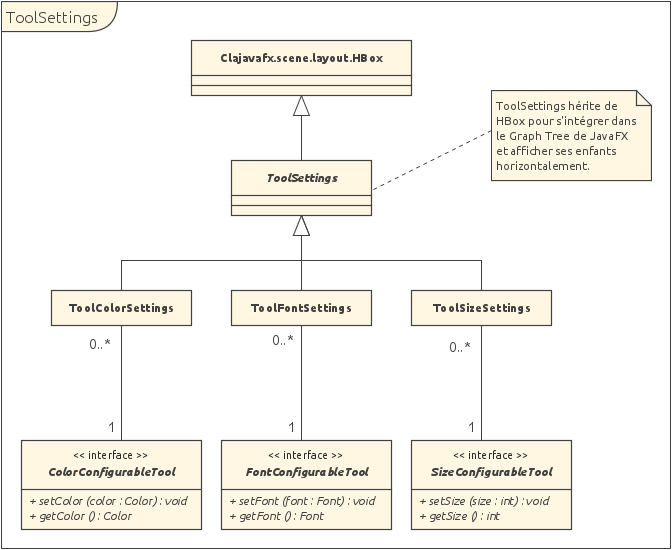
\includegraphics[scale=0.6]{tool_settings.png}
	\label{fig:tool_settings}
\end{figure}

\subsubsection{Pinceau et gomme}
Le pinceau et la gomme ont un comportement et une implémentation quasiment identiques. Dans le programme GEMMS, ce sont les classes \texttt{Brush} et \texttt{Eraser} qui se chargent d'implémenter ces fonctionnalités. Toutes deux héritent d'une classe parente commune: \texttt{LineTool}.
\par
Pour ces deux outils, la problématique était la suivante:
\par
L'événement \texttt{MouseDragged} est déclenché à intervalles réguliers, tant que l'utilisateur effectue cette action. Pour chaque répétition, il est facile de garder trace de la position de la souris au dernier événement et à l'événement actuel. Connaissant ces deux points, il est possible de dessiner une droite.
\par
Pour ce faire, nous avons utilisé l'algorithme de tracé de segment de Bresenham. Mis au point en 1962, cet algorithme permet de déterminer quels pixels sont à colorer pour relier harmonieusement deux points par une ligne droite.
\par
Il existe de nombreuses implémentations de cet algorithme, et nous avons choisi l'implémentation compacte, que l'on peut trouver sur la page allemande de l'article Wikipédia dédié à ce sujet \cite{Bresenham}.
\par
La classe \texttt{LineTool} se charge donc d'implémenter cet algorithme et pour chaque pixel à colorer, elle appelle une méthode abstraite drawPixel que ses sous classes se chargent de définir. Ainsi, \texttt{Brush} dessine un disque correspondant à la taille du pinceau, et \texttt{Eraser} efface un carré de pixels correspondant à la taille de la gomme.
\subsubsection{Pipette}
Le rôle de l'outil pipette (classe \texttt{EyeDropper}) est de permettre à l'utilisateur de choisir une couleur en la prélevant sur un élément existant du document. Il s'agirait typiquement de récupérer la couleur d'un calque \texttt{GEMMSText}, \texttt{GEMMSCanvas} ou \texttt{GEMMSImage}.
\par
Dans le cas d'un texte, la pipette retourne simplement la couleur de celui-ci. Dans le cas d'un objet de type \texttt{GEMMSCanvas} ou d'une \texttt{GEMMSImage}, l'outil lit le pixel exact cliqué par l'utilisateur, si celui-ci se trouve à l'intérieur des bornes du calque sélectionné.
\subsubsection{Modification de texte}
L'outil de modification de texte permet à l'utilisateur de modifier les propriétés d'un calque texte existant. Lorsque il clique dessus, si le clic est effectué dans les bornes visuelles du texte, l'outil ouvre une fenêtre de dialogue invitant à changer le contenu du texte.
\par
Les réglages de couleur et de police de cet outils utilisent la structure expliquée à la section \ref{reglage-outils} en utilisant des objets de type \texttt{ToolColorSettings} et \texttt{ToolFontSettings}.
\subsubsection{Symétries}

Les deux symétries, horizontale et verticale, s'effectuent non pas grâce à un outil qui implémente une interface \textit{Tool} mais grâce à des transformations JavaFX sur les n\oe uds sélectionnes. Cela est principalement dû au fait que les outils implémentant cette interface sont pratiques pour une utilisation avec la souris alors que pour une symétrie, il n'y en a pas besoin. Une symétrie effectue donc une transformation de rotation d'un angle de 180 degrés avec un pivot centré au milieu du n\oe ud et un axe de rotation correspondant à la symétrie. Par exemple, pour la symétrie horizontale, on applique la rotation sur l'axe Y.

Concernant la sérialisation de cette transformation, comme il s'agit de la transformation d'un n\oe ud et que les transformations de JavaFX ne sont pas sérialisables, il faut enregistrer tous les paramètres de la rotation (angle, pivot et axe) afin de pouvoir réappliquer cette transformation lors de la désérialisation.
\subsubsection{Déplacement}
Le rôle de l'outil de déplacement est de pouvoir déplacer un ou des n\oe uds. Pour se faire, il implémente l'interface \textit{Tool} afin de pouvoir déplacer les n\oe uds avec la souris. Il retient la position de la souris lors du clic, calcule un offset lors du déplacement de celle-ci et applique une translation pour chaque n\oe ud selectionné qui consiste à rajouter l'offset aux coordonnées du n\oe ud.

 Il y a deux types de déplacement: celui avec l'alignement automatique et celui sans. Ce dernier, activable via un bouton, permet d'afficher des repères qui traversent le centre du workspace et qui permettent d'aligner un n\oe ud sur ceux-ci. De plus, avec ces repères, il y a un mechanisme d'aimant qui permet, lorsque la souris est assez proche d'un repère d'alignement, d'attirer le n\oe ud selectionné sur lui. Ce mechanisme d'attraction ne marche que s'il n'y a qu'un n\oe ud de selectionné.
\subsubsection{Rotation}
Plusieurs approchent possible pour le méchanisme de rotation mais nous avons finalement opté pour un méchanisme très similaire a l'outil de déplacement : on calcule un offset via la position de la souris et on applique une rotation sur les n\oe uds selectionnés.
\subsubsection{Redimensionnement}
Comme pour l'outil déplacement et l'outil rotation, plusieurs approchent ont été pensées mais celle qui a été retenue est très semblable à la rotation et au déplacement. On calcule un offset avec le déplacement de la souris, on a un certain facteur de grossissement que l'on multiplie à l'offset afin d'obtenir le nouveau grossissement que l'on va appliquer aux n\oe uds.
\subsubsection{Sélection}
\label{sec:selection}
La sélection permet à l'utilisateur de sélectionner une zone du Workspace à l'aide d'un rectangle. Ce dernier peut être déplacé ou recréé si la zone de sélection ne convient pas. Une fois la zone choisie, si le calque courant est un GEMMSCanvas, il possible de supprimer à l'aide de la touche DEL ou de copier à l'aide de la touche CTRL+C.

Pour la suppression de la zone, la classe GraphicsContext qui s'occupe de la partie graphique d'un Canvas offre la méthode clearRect qui permet d'effacer une partie rectangulaire du Canvas (Remplace les pixels présents par des pixels de couleur transparent). Il suffit donc de récupérer la position, la largeur et la hauteur de la zone de sélection et d'utiliser clearRect.

Et enfin pour le copier-coller, voir la section \ref{sec:copiercoller} pour plus d'informations sur son fonctionnement.

\subsubsection{Rognage}
L'outil rognage permet à l'utilisateur de rogner le Workspace à l'aide d'un rectangle. Ce dernier peut être déplacé ou recrée si la zone ne convient pas. Puis lorsque l'utilisateur est satisfait de la zone de rognage, il suffit de cliquer une fois sur le rectangle pour valider.

Le rognage redimensionne simplement le zone d'affichage du Workspace et décale tous les calques présents afin d'afficher la zone choisie par l'utilisateur. Contrairement aux éditeurs comme Gimp ou Paint, le rognage ne coupe pas les calques présents.

Enfin, l'outil rognage et le menu Resize font exactement les mêmes actions.

\subsection{Effets}
La section \og Effect \fg{} permet d'appliquer des effets colorimétriques, régler la transparence et ajouter un flou à un ou plusieurs calques. Chaque calque qui doit être modifié passe par une vérification: s'il n'a aucun effet appliqué, on lui applique trois effets: un ColorAdjust, un SepiaTone et un GaussianBlur permettant d'effectuer respectivement des ajustements de la couleur, un effet sépia, et un flou. Ces effets sont initialement tous réglés pour n'effectuer aucun changement visuel. Ceci permet, lors d'une future modification des effets, de simplement devoir faire varier les paramètres de ces effets.

\subsubsection{Noir et blanc}
Le bouton \og B\&W \fg{} à pour effet de régler la saturation de l'image à sa valeur minimale, donnant pour effet une image en nuances de gris.

\subsubsection{Tint}
Applique une teinture de la couleur sélectionnée à l'image. Ceci est fait en calculant une valeur de la teinte et en l'appliquant à l'effet ColorAdjust.

\subsubsection{Barres glissantes}
Les barres glissantes (\og Sliders \fg{} JavaFX) permettent d'ajuster tous les autres effets implémentés. La transparence règle directement un attribut \og Opacity \fg{} d'un n\oe ud. La saturation, le contraste et la luminosité peuvent être ajustés en modifiant l'effet ColorAdjust. L'effet sépia et le flou ajustent respectivement l'effet SepiaTone et GaussianBlur.

\subsubsection{Remise à zéro}
Le bouton \og Reset \fg{} permet de remettre à zéro tous les effets sur tous les calques sélectionnés, les restaurant à leur état visuel initial.
